\documentclass[main.tex]{subfiles}

\begin{document}

	En primer lugar en base a los datos del filtro solicitado:
	
	\bigskip	
	\centering
	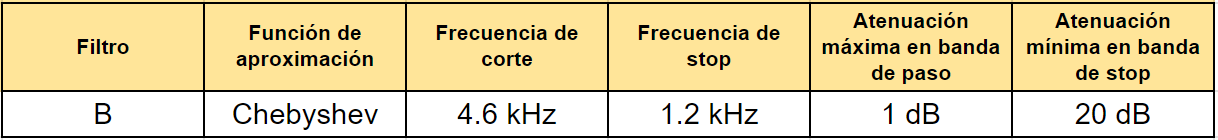
\includegraphics[width=15cm]{./../Imagenes/PlantillaConsigna.png}
	\raggedright	
	\bigskip
	
	Procederemos a realizar la plantilla de atenuación del filtro:
	
	\bigskip	
	\centering
	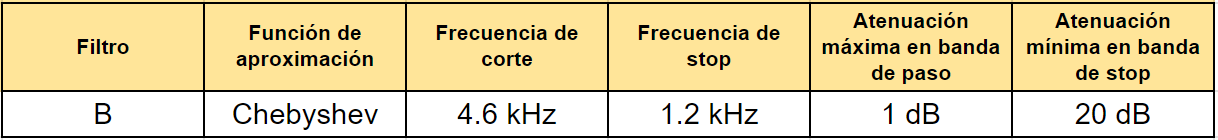
\includegraphics[width=15cm]{./../Imagenes/PlantillaConsigna.png}
	\raggedright	
	\bigskip
	
	Luego, debido a que nos encontramos en presencia de un filtro pasa altos, debemos convertir los parametros de la plantilla a un filtro pasa bajos prototipo, de la siguiente forma:
	
	\bigskip	
	\centering
	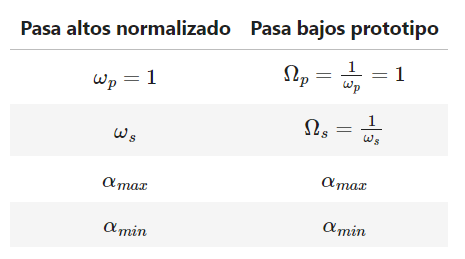
\includegraphics[width=15cm]{./../Imagenes/ConversionHPLP.png}
	\raggedright	
	\bigskip
	
	Todo este desarrollo tambien se puede realizar de forma "numerica" en Python, donde se verficara que se obtendran los mismo resultados. Esta simulacion numerica se puede encontrar en el siguiente link de nbviewer: 
	
\end{document}	